\section{Interprétation et exploitation}

\begin{frame}
\frametitle{Interprétation et exploitation}
\framesubtitle{Apport du modèle FHN}
\begin{itemize}
  \item Sa simplicité permet d'isoler les mécanismes essentiels de l'excitabilité.
  \item Il permet la simulation de phénomènes complexes comme les ondes spirales.
  \item Ces ondes spirales sont responsables d'arythmies.
\end{itemize}
\end{frame}

\begin{frame}
\frametitle{Interprétation et exploitation}
\framesubtitle{Application à la défibrillation cardiaque}
\begin{figure}
\caption{Dissolution du noyau d'une onde spirale}
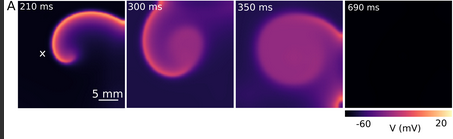
\includegraphics[width = \linewidth]{Figures/Breakup.png}
\source{(2023) Dissolution of spiral wave’s core using
cardiac optogenetics. PLoS Comput Biol 19(12):
e1011660}
\end{figure}
\end{frame}

\begin{frame}
\begin{center}
\textbf{Merci de votre attention}
\end{center}
\end{frame}